%
% teil2.tex -- Beispiel-File für teil2 
%
% (c) 2020 Prof Dr Andreas Müller, Hochschule Rapperswil
%
% !TEX root = ../../buch.tex
% !TEX encoding = UTF-8
%
\section{Audioanalyse
\label{sonogramm:section:teil2}}
\rhead{Audioanalyse}
In diesem Abschnitt werden wir mit Hilfe des Sonogramms ein Musikstücks
analysieren und versuchen die gespielten Noten zu rekonstruieren.

Wir nehmen dafür einen fünf Sekunden langen Abschnitt vom Lied
Dern Kala von Khruangbin.
Um uns die Arbeit zu vereinfachen, verwenden wir ein Audiosignal, in
dem nur die Gitarre zu hören ist.
Abbildung \ref{sonogramm:dernTime} zeigt das Audiosignal in der Zeit.
Man kann die Stellen, and welchen Töne gespielt wurden, gut erkennen.
Um nun die Tonhöhen zu erkennen brauchen wir das Sonogram.
Wie das Tonsystem aufgebaut ist, wird in Abschnitt \ref{autotune:section:tonsystemUndStimmung}
genauer beschrieben.
\begin{figure}
    \centering
    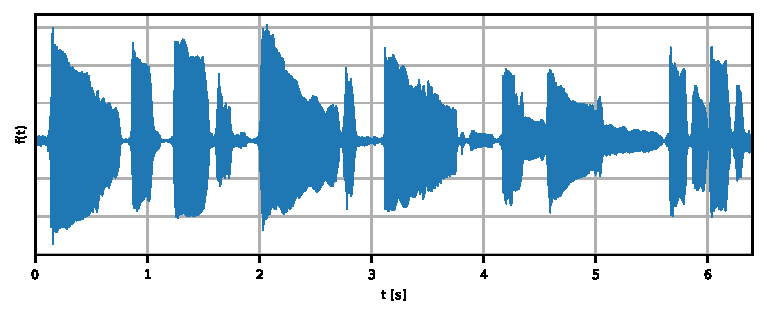
\includegraphics{papers/sonogramm/images/audioTimeDern.pdf}
    \caption{Audo Spur für die Tonanalyse.
    \label{sonogramm:dernTime}
    }
\end{figure}

Eine grundsätzliche Entscheidung, die wir treffen müssen
ist die Zeitliche Auflösung, die wir haben möchten, welche 
dann auch unsere Frequenzauflösung beeinflusst.
Für unser Stück haben wir den Vorteil, dass jeweils nur einzelne
Töne gespielt werden, wir müssen also nicht zwei Töne zur selben 
Zeit erkennen.
Die benötigte Zeitauflösung können wir anhand der Geschwindigkeit des Lieds abschätzen.
Diese beträgt 83 Schläge pro Minute mit einem 4/4 Takt, also jeweils alle 0.69 Sekunden ein viertel Takt.
Möchten wir sechzehntel Noten erkennen darf die STFT über maximal 0.17 Sekunden
angewendet werden.
Damit die sechzehntel Noten nicht nur in einem Segment zu sehen sind teilen
wir die 0.17 Sekunden nochmals durch zwei.
Das liefert uns bei einer Abtastfrequenz von 44100 Hz eine ungefähre Segmentlänge von 
3800 Samples. 
Nach einem Bisschen Ausprobieren ergibt sich 4000 als eine geeignete Segmentlänge.

Um die Leckfrequenzen verwenden wir ein Hamming Fenster.
Somit resultiert das Sonogramm in Abbildung \ref{sonogramm:dernSono}.


\begin{figure}
    \centering
    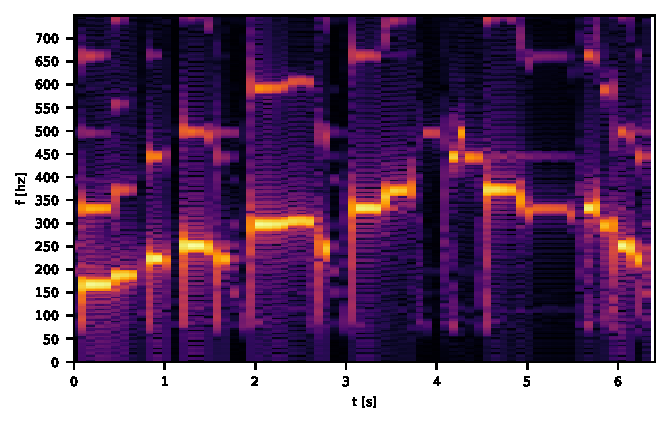
\includegraphics{papers/sonogramm/images/dernSono1.pdf}
    \caption{Sonogram des Abschnitts von Dern Kala.
    \label{sonogramm:dernSono}
    }
\end{figure}

Die gespielten Töne könne wir nun anhand der Frequenzen 
der Peaks in den Segmenten errechnen.
Abbildung \ref{sonogramm:dernSonoPeaks} zeigt TODO

\begin{figure}
    \centering
    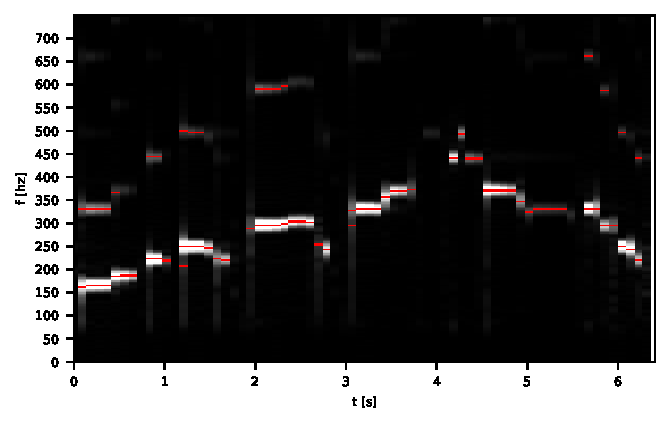
\includegraphics{papers/sonogramm/images/dernSonoPeaks.pdf}
    \caption{Gefundene Frequenzen in Rot eingezeichnet. Bei gewissen 
    Segmenten werden Peaks auch bei der doppelten Frequenz gefunden.
    Dies sind die Obertöne der gespielten Gitarrensaiten.
    \label{sonogramm:dernSonoPeaks}
    }
\end{figure}

\subsection{De finibus bonorum et malorum
\label{sonogramm:subsection:bonorum}}


